\chapter{INTRODUCTION and opening remarks} \label{intro}

We don't make the Chapter titles in All Caps Automatically because it is easier for you to type your Chapter Titles in uppercase than for those that need to have mixed case in their titles to find the correct command in the ufthesis.cls file and change it there. \renewcommand*{\thefootnote}{\fnsymbol{footnote}}\footnote{an un-numbered footnote - this is how you tell the readers that this chapter was previously published and then cite the Journal where it was published} We don't recommend that you change much of anything in the class file unless you're absolutely sure of what your are doing.\renewcommand*{\thefootnote}{\arabic{footnote}}\setcounter{footnote}{0}\footnote{and now we're back to normal footnote marking} 

\section{The Section Command Text Should Be in Title Case}

 Title case is where all principal words are capitalized except prepositions, articles, and conjunctions.  \cite{green2008wrinkle}

\subsection{Subsection Commands Are Also in Title Case}
The difference, of course, are the second level headings are left-aligned

\subsubsection{Subsubsections are in sentence case}
The third level subheadings are left-aligned but in sentence case. Only the first letter and any proper nouns are capitalized. \cite{strickler1998contamination}

\subsubsection{If you divide a section, you must divide it into two, or more, parts}

{\bf Paragraph headings.} There is no official fourth level heading. Do not use the Paragraph heading feature in LaTeX, simply apply the bold characteristic to the first few words of a paragraph followed by a colon or period.

\subsection{I Need Another Second Level Heading in This Section}

Aliquam mi nisi, tristique at rhoncus quis, consectetur non mi. Phasellus blandit quam ligula, a viverra lacus commodo at. In iaculis nisl vel pretium sollicitudin. In efficitur massa vel elit sollicitudin, vel auctor sapien cursus. Proin feugiat sapien a mi tempus;

 $ X-X'=D+D'$

 in consequat augue cursus. Nulla sed sagittis purus. Nunc eu consequat orci, eu laoreet enim. Ut euismod tincidunt sem, eget lacinia dui luctus eu. Aliquam mi augue, faucibus id semper vitae, porta ac ligula. Morbi sed ultrices odio. Mauris id luctus ex. Nulla ac libero dictum, interdum turpis lacinia, scelerisque leo. Praesent varius orci ac eros varius pharetra.

\section{Image Handling in XeLaTeX}

One of the biggest reasons for switching from the dvipdfm/dvipdfmx methods of compiling is the improved image handling capabilities. EPS, Bit-mapped, PDF, JPG, and PNG formats work well with the xelatex process.

\subsection{The Traditional EPS Format}

EPS format is the traditional format for LaTeX, but EPS files can be very large and many programs can't create or view these images. There are many programs that are used to interpret data and output the results as an EPS format image. It has been my experience that there are bounding box problems with these figures. On many occasions we have opened the image in Adobe Photoshop and, without making any changes, saved the document as a Photoshop EPS file, re-compiled the document, and the image worked correctly, so if you are having problems with an EPS image not showing in your document correctly, try this fix first.


\begin{figure}[htbp]
  \centering
    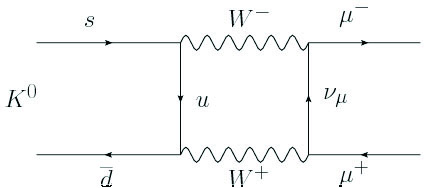
\includegraphics[width=5in]{images/diagram}
    \caption[EPS format diagram. Note: no filetype is designated by adding an extension.]{EPS format diagram. Note: no filetype is designated by adding an extension. The file type is determined and the correct procedure is automatically chosen by xelatex.}
\end{figure}


Quisque malesuada a leo eget ullamcorper. Curabitur ut aliquam quam. Nam quis quam id mauris aliquam blandit porttitor sit amet quam. Donec ut erat eleifend turpis finibus pulvinar.

\subsection{Bitmapped Images Work As Well}

Bitmapped images are a standard file type on PCs, but these files are also usually very large so compressed images may be a better alternative.

\begin{figure}[htbp]
  \centering
    \includegraphics[width=5in]{images/eagle}
    \caption[BMP format drawing. Note: no filetype is designated by adding an extension.]{BMP format drawing. Note: no filetype is designated by adding an extension. The file type is determined and the correct procedure is automatically chosen by xelatex.}
\end{figure}

Morbi hendrerit risus nec quam posuere viverra. Donec quis tellus faucibus, molestie arcu sed, congue urna. Duis eget neque ac libero pulvinar porta eget et magna. Donec a magna eu eros suscipit cursus ac vitae nisl. Vivamus ligula purus, congue sed tortor blandit, ultrices egestas nisl.

\subsection{Not to Mention PDF}

It is often very handy to be able to include a pdf file as an image. By using XeLaTeX this is usually just matter of setting the size, or scale properties correctly.

\begin{figure}[htbp]
  \centering
    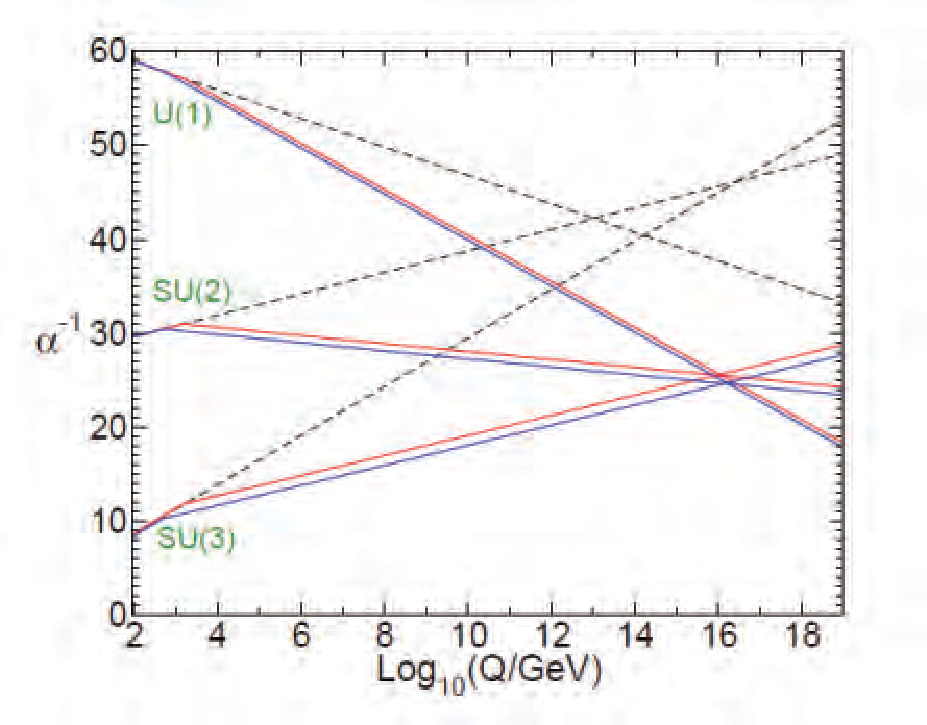
\includegraphics[scale=1.0]{images/graph.pdf}
    \caption[PDF format graph. Note: no filetype is designated by adding an extension.]{PDF format graph. Note: no filetype is designated by adding an extension. The file type is determined and the correct procedure is automatically chosen by xelatex.}
\end{figure}

Nulla mattis augue lacus. Nam non lectus dolor. Cras ac quam vel justo elementum vestibulum. Integer vulputate pulvinar lacus sit amet pulvinar.

\subsection{JPG Is Absolutely Necessary}

For photographs, JPG is the most common format. This format is a fraction of the size of Bit-mapped images and can deliver very good quality at a much smaller overhead. Vestibulum eu lectus vel orci dictum vehicula. Proin id maximus dolor. Integer augue ante, pulvinar ac erat vitae, porttitor ullamcorper libero. \cite{l2012wrinkle}

\begin{figure}[htbp]
  \centering
    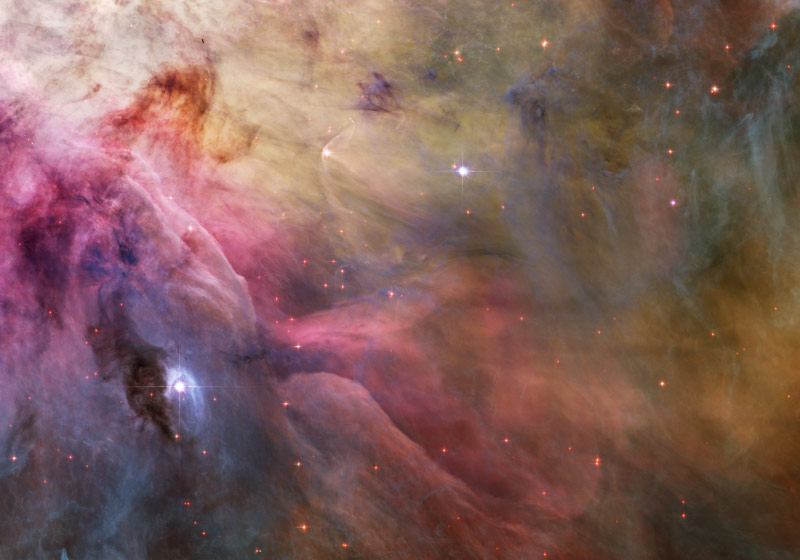
\includegraphics[width=5in]{images/nebula}
    \caption[JPG format image. Note: no filetype is designated by adding an extension.]{JPG format image. Note: no filetype is designated by adding an extension. The file type is determined and the correct procedure is automatically chosen by xelatex.}
\end{figure}

Nunc blandit scelerisque velit, ac facilisis dui finibus et. Sed facilisis tortor vel commodo luctus. Donec est felis, malesuada id nibh in, accumsan malesuada lectus. Sed lobortis volutpat felis, vitae aliquet augue congue id. Fusce ut odio tincidunt, condimentum nulla vel, pharetra arcu.

\subsection{PNGs Will Help Make Files Smaller}

PNG files are even smaller than JPGs and are very good when text and images are combined.

\begin{figure}[htbp]
  \centering
    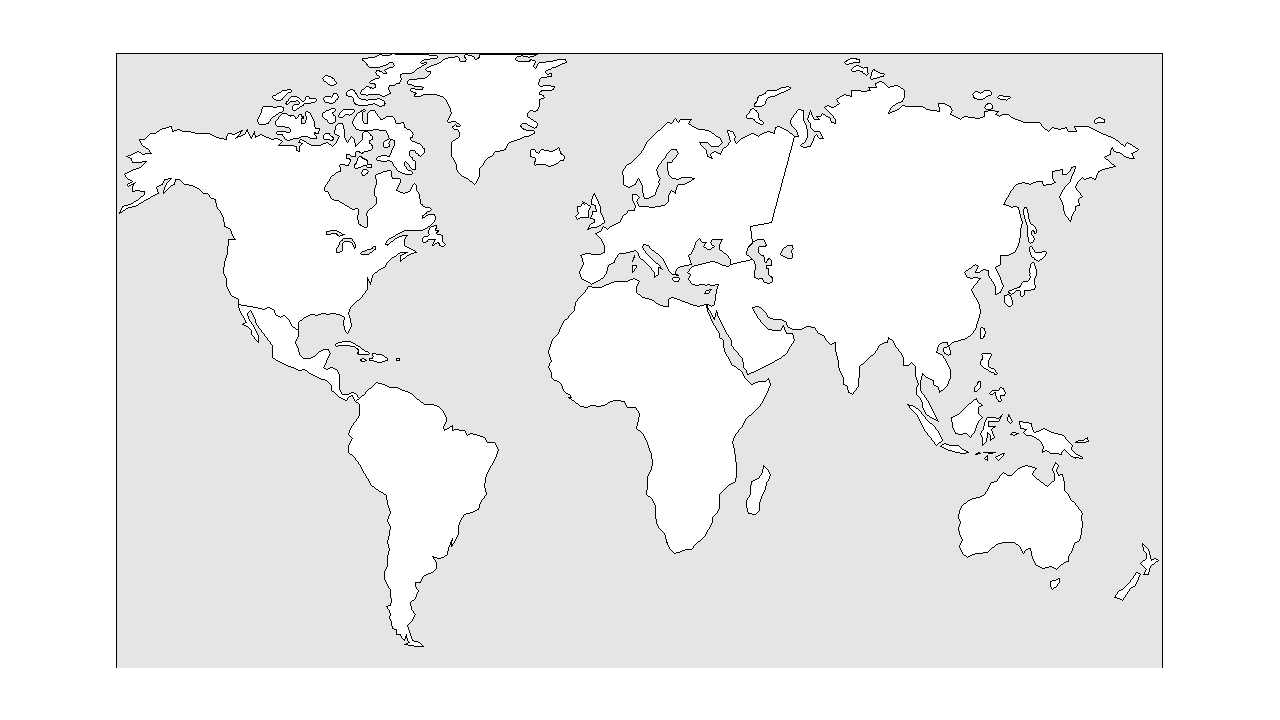
\includegraphics[width=5in]{images/theworld}
    \caption[PNG format map. Note: no filetype is designated by adding an extension.]{PNG format map. Note: no filetype is designated by adding an extension. The file type is determined and the correct procedure is automatically chosen by xelatex.}
\end{figure}



Aenean condimentum libero sed mi porta, tempus ullamcorper lectus venenatis. Aliquam in diam dolor. Maecenas tempus consectetur sem et pulvinar. Aenean aliquam at metus ut hendrerit. Vivamus molestie ac neque eu luctus. Nam convallis maximus quam non lobortis. Fusce sit amet lorem et massa convallis aliquet at sit amet nulla. Suspendisse nec ex elit. Aenean gravida, sapien vitae congue commodo, urna turpis ornare libero, at cursus risus libero in erat. \cite{Rust94}

\section{GIF, TIF, and Others}

Other file formats have not been successful, with or without file extensions. The tests have not been exhaustive so if you have a different type, give it a try. GIF, and TIF both do NOT work at this time. The next image demonstrates how to use multiple images as a single figure. Notice, there is a single caption for ALL figures and that caption starts with a discription of the ENTIRE figure before breaking off into the subfigure descriptions.

\begin{figure}[htbp]
     \centering
   \mbox{
      \subfigure [] {
\includegraphics[scale=0.6]{images/mouse}} \qquad
      \subfigure []{
\includegraphics[scale=0.6]{images/mouse}} \qquad
     }
    \mbox{
      \subfigure [] {
\includegraphics[scale=3]{images/cat}} \qquad
      \subfigure [] {
\includegraphics[scale=0.6]{images/mouse}} \qquad
      }
    \caption[Tom and Jerry]{Tom and Jerries. This caption demonstrates how the sub-captions are left out of the List of Figures, but included in the figure itself. A) Tom the first; B) Tom the second; C) Jerry; D) Tom the third.}
    \label{mice}
  \end{figure}


Aliquam mi nisi, tristique at rhoncus quis, consectetur non mi. Phasellus blandit quam ligula, a viverra lacus commodo at. In iaculis nisl vel pretium sollicitudin. In efficitur massa vel elit sollicitudin, vel auctor sapien cursus. Proin feugiat sapien a mi tempus, in consequat augue cursus. Nulla sed sagittis purus. Nunc eu consequat orci, eu laoreet enim. Ut euismod tincidunt sem, eget lacinia dui luctus eu. Aliquam mi augue, faucibus id semper vitae, porta ac ligula. Morbi sed ultrices odio. Mauris id luctus ex. Nulla ac libero dictum, interdum turpis lacinia, scelerisque leo. Praesent varius orci ac eros varius pharetra.



Nunc blandit scelerisque velit, ac facilisis dui finibus et. Sed facilisis tortor vel commodo luctus. Donec est felis, malesuada id nibh in, accumsan malesuada lectus.
\begin{itemize} %
    \item WinEDT: This text editor is recommended for use editing \TeX-files as it has many useful built in macros and is easy to use  %
    \item This program can be found and downloaded here: \url{http://www.winedt.com/} %
    \item The GIMP (GNU Image Manipulation Program) %
    \begin{itemize}%
        \item A freeware graphics editing program for picture editing and file conversions %\vspace{-12pt}%
        \item Comparable to Adobe Photoshop %\vspace{-12pt}%
        \item Can be downloaded here: \url{http://www.gimp.org/}%
    \end{itemize}
    \item A good reference of \LaTeX 2\ensuremath{\epsilon} commands%
    \begin{itemize}
        \item This should be included on the ETD website here: \url{http://etd.helpdesk.ufl.edu/tex.php}
    \end{itemize}
\end{itemize} %


Sed lobortis volutpat felis, vitae aliquet augue congue id. Fusce ut odio tincidunt, condimentum nulla vel, pharetra arcu. In ultricies libero diam, nec rutrum magna vehicula nec. Praesent dictum eros sit amet turpis ultricies, eleifend condimentum dui imperdiet. Donec congue urna ante, id rutrum mi commodo a. Vivamus id tincidunt nunc. Morbi id lacus ut augue ultricies convallis. Duis a lectus quis ante pretium scelerisque nec nec nisi. In id porta justo, at euismod diam. Suspendisse vel tempus arcu. Praesent vel cursus nisi, ac rhoncus odio.

